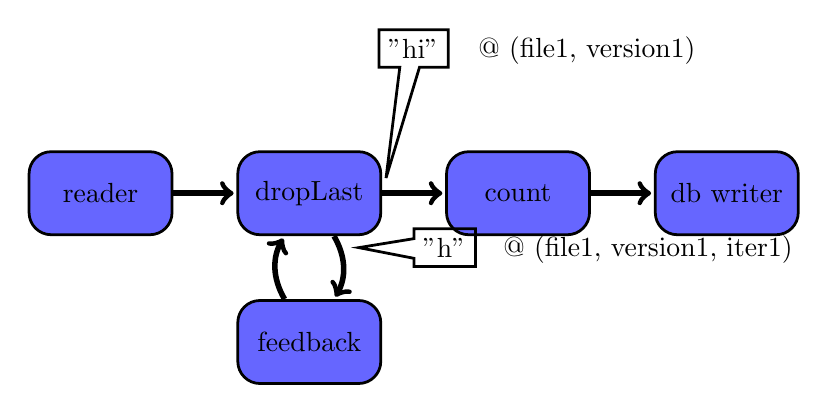
\begin{tikzpicture}[node distance = 0.8cm, auto]
\usetikzlibrary{shapes,arrows}
\usetikzlibrary{positioning}

\tikzstyle{operator} = [rectangle, draw, fill=blue!60, text width=4.5em, text centered, rounded corners = 8pt, minimum height=30pt, line width=1pt]
\tikzstyle{callout} = [draw, rectangle callout, callout relative pointer={#1}, line width=1pt]

    \node [operator] at (0, 0) (reader) {reader};
    \node [operator, right = of reader] (filter) {dropLast};
    \node [operator, right = of filter] (count) {count};
    \node [operator, below = of filter] (feedback) {feedback};
    \node [operator, right = of count] (writer) {db writer};

    \draw [thick,->,shorten >=1pt, line width=2pt] (reader) -- (filter) ;
    \draw [thick,->,shorten >=1pt, line width=2pt] (filter) -- (count)
       node[callout={(-0.3,-40pt)}, midway,above = 45pt] {"hi"} node[midway,above= 45pt, shift={(2.2,-0.1)}] {@ (file1, version1)}; 
     \draw [thick,->,shorten >=1pt, line width=2pt] (count) -- (writer); 
    \draw [thick,->,shorten >=1pt, line width=2pt] (filter) to  [bend left]  (feedback)  
      node[callout={(-0.7,0pt)}, above right  = 20pt , shift={(0.5,-0.1)}] {"h"} node[ above right  = 20pt , shift={(1.5,-0.2)}] {@ (file1, version1, iter1)}; 
     \draw [thick,->,shorten >=1pt, line width=2pt] (feedback) edge  [bend left]  (filter); 
\end{tikzpicture}
